\chapter{Control for \SB{} Locomotion}
\label{controls}

\section{Basic Locomotion Concepts for a Icosahedron Tensegrity Robot}
\label{basic_locomotion}

Locomotion for tensegrity structures like \SB{} is achieved by deforming the structure in a way in which moves the system's center of mass to an unstable configuration, tipping the robot over.
This deformation is usually achieved by either changing the length of the main cable network on the outside of the robot~\cite{sabelhaus2015system,kim2014rapid} or by adding additional cables which run through the structure connecting non-parallel rods~\cite{caluwaerts2014design}.
For the rest of this section, deformation is assumed to be done by actuating the main cable network on the outside of the robot since this is how \SB{} is deformed.

% \SB{} is a tensegrity structure is the shape of an icosahedron.
An regular convex icosahedron is a geometric shape consisting of eight equilateral triangle interlaced with twelve isosceles triangles.
In a passively sable configuration, the bottom of an icosahedron will be resting on either an equilateral or a isosceles triangle.
Utilizing this knowledge, the most simple method for moving the center of mass of an icosahedron can be obtained by changing the length of one side of the bottom triangle to near zero.
This will always move the center of mass to an unstable configuration by effectively reducing the bottom triangle, as seen if figure~\ref{fig:single_flop}, which will cause the robot to transition to another face.
However, this simple control method is not always obtainable on a real robotic system due to limitation on actuation or design methodology.

\label{hand_stepwise}
\begin{figure}[thpb]
      \centering
      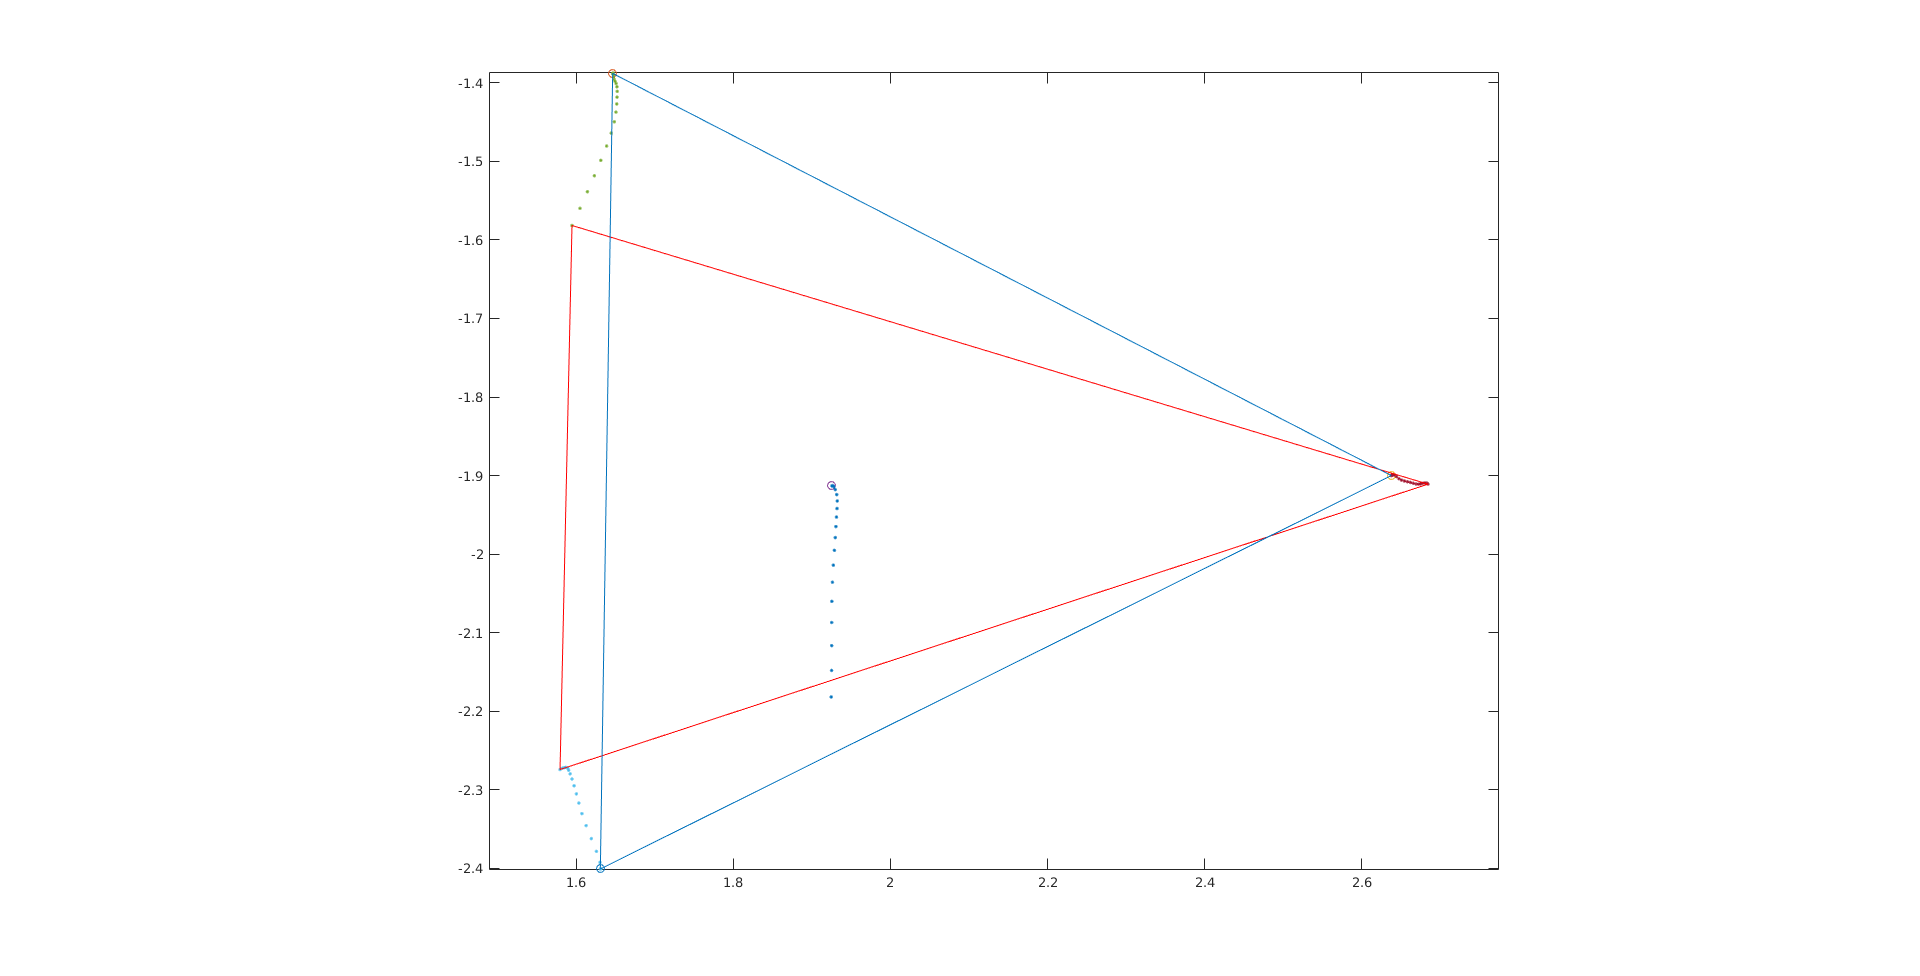
\includegraphics[width=1\columnwidth]{tex/img/Single_flop_bottom_triangle}
      \caption{This is XY data of the bottom triangle of a NTRT simulation of \SB{} performing a single face transition by changing only one side of the bottom triangle.
      No other cable on the system is being actuated during this simulation.
      The red triangle is the bottom triangle at the start of the simulation. 
      The centralized circle represents the center of mass (CoM) of the entire simulated \SB{}. 
      The blue triangle is the configuration where the CoM moves out of the bottom triangle and the robot begins to transition to another face.
      Thus, under ideal conditions and actuation limits, a \SB{} like structure can perform a face transition by the changing of a single cable.}
      \label{fig:single_flop}
\end{figure}

\SB{} is an underactuated icosahedron tensegrity robot.
Of the 24 connection cables, \SB{} only has 12 which are actively actuated and the other cables are passive as discussed in section~\ref{design}.
Therefore, there is a unique pattern of cables, and some care is needed when choosing this pattern for locomotion as there are some patterns where forward rolling is not achievable. 

% There has been many open loop control techniques that explored this concept through the use of form finding static poses~\cite{}\textcolor{red}{bliss, mirats-tur}.
% Their simulation results show some very promising results for locomotion of variou
% xKim et al~\cite{kim2015robust} developed a method which address some of these issues, but requires .... \textcolor{red}{something non-ideal}.
% However, these techniques do not generalize well to ill-formed robot parameters between simulation and a physical robot, and usually constrain the search space to small manifolds for valid structure configurations.
% When the manifolds are expanded, the search space can become very large resulting in slow results that require a large number of 

% \textcolor{blue}{write about Atil's work and Brian's.}


%Another interesting point could be made about there being two classes of tensegrity robots.  Many of the early approaches stemmed directly out of the modeling and mathematics of static tensegrity structures, which used low-creep cables for stability, and such designs result in very small manifolds of valid structures, with many of the changes in cables lengths resulting in the robot becoming unstable and collapsing as there was no valid equilibrium pose.

\section{Hand-Tuned Stepwise Controller}
The initial controller developed for \SB{} was a basic open loop, hand tuned controller.
Motor position commands where systematically found through experimentation which moved the robot into a kinematically unstable configuration for each of the six faces mentioned in section~\ref{basic_locomotion}.
Under normal conditions on flat ground, when the system starts on an equilateral triangle the forward momentum of the structure after deformation will push it through the isosceles triangle and come to rest on another equilateral triangle.
Using this assumption, only six different kinematic configurations where implemented.
To automate this process, enabling the system to detect which face it resided on was necessary.
A simple K-nearest neighbor algorithm was implemented on recorded IMU data for each equilateral triangle face of \SB{}.
Since the faces are discrete enough, one hundred percent classification was found.
With this information, a basic open loop controller was written that used the detected face as an input and commanded the correct motor commands for the kinematically unstable configuration to transition the robot to the next face.
Once the robot acted the kinematically unstable configuration, all motor commands were set back to their starting configuration.
This ensured correct detection and transition time for the next cycle.
The hand-tuned stepwise controller has two main states, a detect and move state and a relax state as seen in~\ref{fig:stepwise_fsm}.
The transition between each state is time based, where the timing between states was empirically obtained to ensure transition and dynamic settling.

\label{hand_stepwise}
\begin{figure}[thpb]
      \centering
      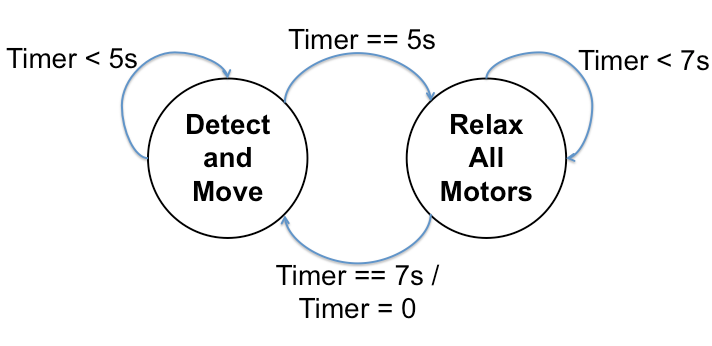
\includegraphics[width=0.7\columnwidth]{tex/img/Stepwise_state_machine/Slide1_fixed}
      \caption{Time based state machine which automates the our hand-tuned stepwise controller. Timers are used to allow for dynamic settling before the next action is taken.}
      \label{fig:stepwise_fsm}
\end{figure}

\section{Learned Neural Net Controller using Guided Policy Search}
\label{learned_controllers}


\section{Central Pattern Generator Controller}
\label{cpg_controller}

\section{Dynamic Rolling}
\label{dyncamic_rolling}